\section{Similarity selection}
\label{sec:gc:simulations}

Given a set $\mathcal{S}$ of various graph pairs, we would like to select 
$(G^i,G^j) \in \mathcal{S}$ where $(G^i,G^j)$ is the most similar graph pair. 
To be more specific, we wish to select graph $\hat{G^i}$ where $\hat{G^i}, i 
\in \{1,...,k\}$ is most similar to the ``base'' graph $\hat{G}$. $\hat{G^i}$ 
is selected out of $k$ given graphs each associated with a vector 
$\overrightarrow{d^{i}}$ of their differences (Again, $i \in \{1,...,k\}$). 
Each element $\overrightarrow{d^{i}_m}$ for $m \in 
\{1,...,6\}$ corresponds to one of the six summarization methods listed 
earlier in Section~\ref{sec:gc:methods}. 
We propose the following methodology to select the most similar graph pair:

\tablespacing
\begin{enumerate}
	\item Compare each difference metric $\overrightarrow{d^{i}_m}$ against 
	$\overrightarrow{d^{i'}_m}$ for all $m \in \{1,...,6\}$ and $i,i' \in 
	\{1,...,k\}$ where $i \neq i'$. 
	\item Select the index $i$ which has the most number of smallest 
	differences. In other words, find
	$$\max\limits_{i \in \{1,...,k\}} 
	\sum\limits^{6}_{m=1} \textbf{1}_{\overrightarrow{d^{i}_m} > 
	\overrightarrow{d^{i'}_m}} \ \text{where} \ i \neq i' \in \{1,...,k\}$$
\end{enumerate}
\bodyspacing

Aside from returning the most similar graph pair, the proposed similarity 
selection method further eliminates the need to normalize the resulting 
difference metrics, which will not be on the same scale within 
$\overrightarrow{d_{i,j}}$, as it compares each metric to its own metric rather 
than computing an aggregate ``difference'' between graphs $\hat{G}^i$ and 
$\hat{G}^j$. In the next Section~\ref{sec:gc:simulations:algorithm}, we 
demonstrate the viability of this strategy with a simulation study. 
This method is later applied in Chapter~\ref{ch:usage} to compare the visual 
graph (output from the VS) and the various correlation graphs (with correlation 
coefficients explained in Section~\ref{sec:intro:correlation})
The similarity selection method is coded in 
Appendix~\ref{sec:appendicies:gc:similarity}.

\subsection{Simulation study}
\label{sec:gc:simulations:algorithm}

We now perform a simulation study to demonstrate the viability of this 
selection strategy. Let $G=(V,E)$ be a base graph with $|V|=20$ nodes and 
$|E|=50$ edges. The idea is to generate two random graphs $G^1, G^2$ from $G$ 
such that $\text{diff}(G,G^1) << \text{diff}(G,G^2)$ or vice versa. 
In other words, one graph should clearly be similar to $G$ while the other is 
very dissimilar to $G$. This is achieved by randomly swapping $\frac{|E|}{5} = 
10$ and $|E| = 50$ edges from $G$ to build $G^1$ and $G^2$, respectively. 
The random swapping algorithm is as follows:

\tablespacing
\begin{algorithm}[H]
	\caption{Random edge swapping}\label{alg:gc:simulations:swapping}
	\begin{algorithmic}[1]
		\Procedure{}{$G=(V,E)$ is the ``base'' graph. Generate a 
		random graph $G^i=(V,E^i)$ by randomly swapping $e$ edges of $G$.
		Let $p_k$ be the probability of randomly selecting node $V_k$ with the 
		given PDF. }
		\State $G^i \gets G$
		\State \textbf{loop from} $f=1$ \textbf{to} $e$:
		\State \indent Select $E_i$ uniformly at random and delete from $G^i$
		\State \indent Select $V_i$ uniformly at random
		\State \indent Select $V_j$ at random where 
		$p_k = \frac{deg(V_k)}{\sum\limits_{x=1}^{|V|} deg(V_x)} \ \forall \
		k \in \{1,...,|V|\}$
		\State \indent \textbf{while} ($V_i = V_j$ \textbf{or} $(V_i,V_j)$ 
		exists):
		\State \indent \indent Reselect $V_j$ at random with the same PDF $p$*
		\State \indent Add edge $(V_i,V_j)$ to $G^i$
		\State \textbf{return} where($p==\min{(p)}$)
		\EndProcedure
	\end{algorithmic}
	*Selecting the second node in this manner ensures that the assortativity 
	coefficient continues to evolve as the swapping proceeds. 
\end{algorithm}
\bodyspacing

\noindent Naturally, $G^1$ should be more similar to $G$ since less 
edges are being swapped than in $G^2$. The differences between the pair 
$(G,G^i)$ for $i \in \{1,2\}$ are computed given the summarization 
methodologies discussed in Section~\ref{sec:gc:methods}, and the most similar 
graph pair is selected with the similarity selection method described earlier. 
The results are then recorded for 1000 trials, and an average is taken. 
The code for the simulation study may be found in 
Appendix~\ref{sec:appendicies:gc:simulations}. 

\subsection{Results}
\label{sec:gc:simulations:results}

The results are as follows:

\tablespacing
\begin{longtable}{p{0.15\linewidth} p{0.25\linewidth} 
p{0.15\linewidth} p{0.15\linewidth}}
	
	% First page heading
	\caption[Summary of similarity selection simulation results.]{A summary of 
	the  similarity selection simulation results as described in 
	Section~\ref{sec:gc:simulations:algorithm}. The table summarizes the 
	probability of selecting graphs $G^1$ and $G^2$ with the given number of 
	swaps. (C) is an abbreviation for (CONTROL)} 
	\label{tab:gc:simulations}\\
	\toprule
	\textbf{Distance} & \textbf{Number of swaps} & 
	\textbf{Prob}($G^1$) & \textbf{Prob}($G^2$) \\
	\midrule
	\endfirsthead
	
	% Future page heading
	\caption[]{(continued)}\\
	\toprule
	\textbf{Distance function} & \textbf{Number of swaps} & 
	\textbf{Prob}($G^1$) & \textbf{Prob}($G^2$) \\
	\midrule
	\endhead
	
	% Page footer
	\midrule
	\multicolumn{4}{r}{(Continued on next page)}\\
	\endfoot
	
	% Last page footer
	\bottomrule
	\endlastfoot
	
	Euclidean & $G^1: 10, G^2: 10$ (C) & 
	0.54 & 0.46 \\
	
	& $G^1:10, G^2: 50$ & 0.885 & 0.115 \\
	
	\cmidrule[0.1pt](l{0.5em}r{0.5em}){1-4}	
	
	L1 & $G^1: 10, G^2: 10$ (C) & 
	0.532 & 0.468 \\
	
	& $G^1:10, G^2: 50$ & 0.886 & 0.114 \\
	
	\cmidrule[0.1pt](l{0.5em}r{0.5em}){1-4}	

	L2 & $G^1: 10, G^2: 10$ (C) & 
	0.541 & 0.459 \\
	
	& $G^1:10, G^2: 50$ & 0.885 & 0.115 \\
		
\end{longtable}
\bodyspacing

\noindent It is clear, then, that the proposed similarity selection method is 
likely to properly select the most similar graph pairs on average. To visualize 
the similarity between 10 vs 10 and 10 vs 50 swaps, please review 
Figures~\ref{fig:gc:sim10vs10} and~\ref{fig:gc:sim10vs50}, which plot the 
graphs resulting from the swaps in the final simulation trial. Since the 
control and the true simulations were run separately and each trial seeded with 
its trial number, the base graph and $G^1$ (which has 10 swaps in each 
simulation) are, expectedly, the same. It is $G^2$ that differs.

\begin{figure}[htb]
	\begin{center}
		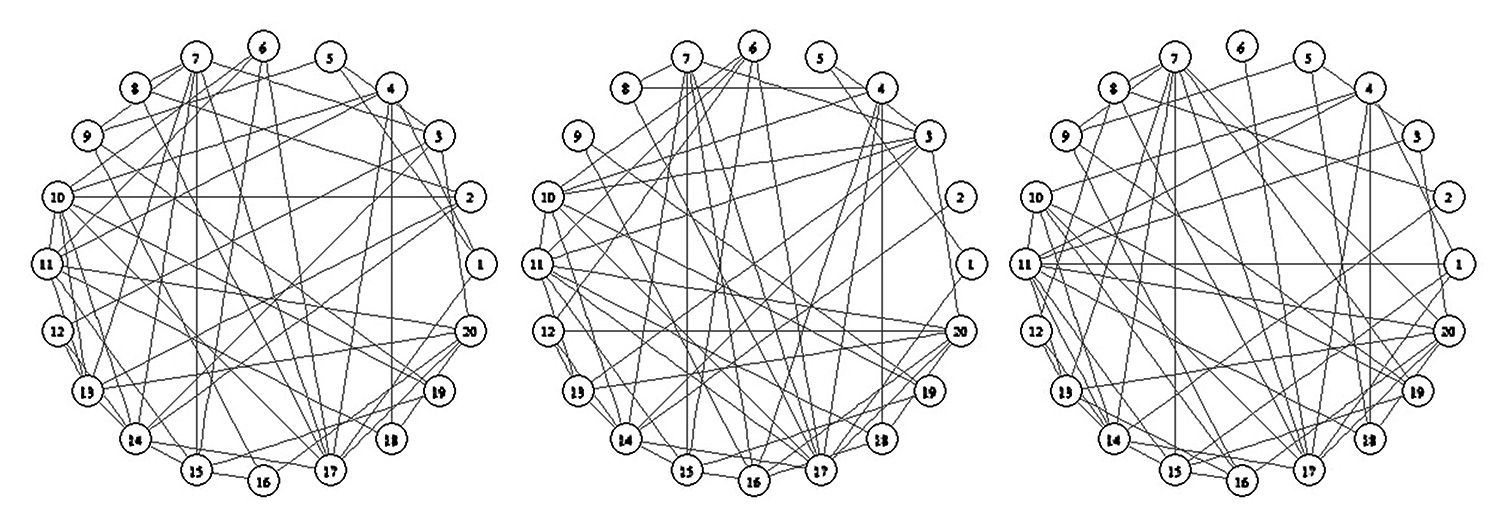
\includegraphics[width=1\linewidth]{ch-gc/figures/sim_10vs10}
		\caption[Random graphs with 20 nodes and 50 edges. Edges have been 
		swapped 10 times each.]{\textit{Left:} Base graph $G(V,E)$ with $V=20$ 
		nodes and $E=50$ edges. \textit{Middle and Right:} Two random graphs 
		built from $G$ by randomly swapping 10 edges. Distance: L2. Seed: 1000}
		\label{fig:gc:sim10vs10}
	\end{center}
\end{figure}

\begin{figure}[htb]
	\begin{center}
		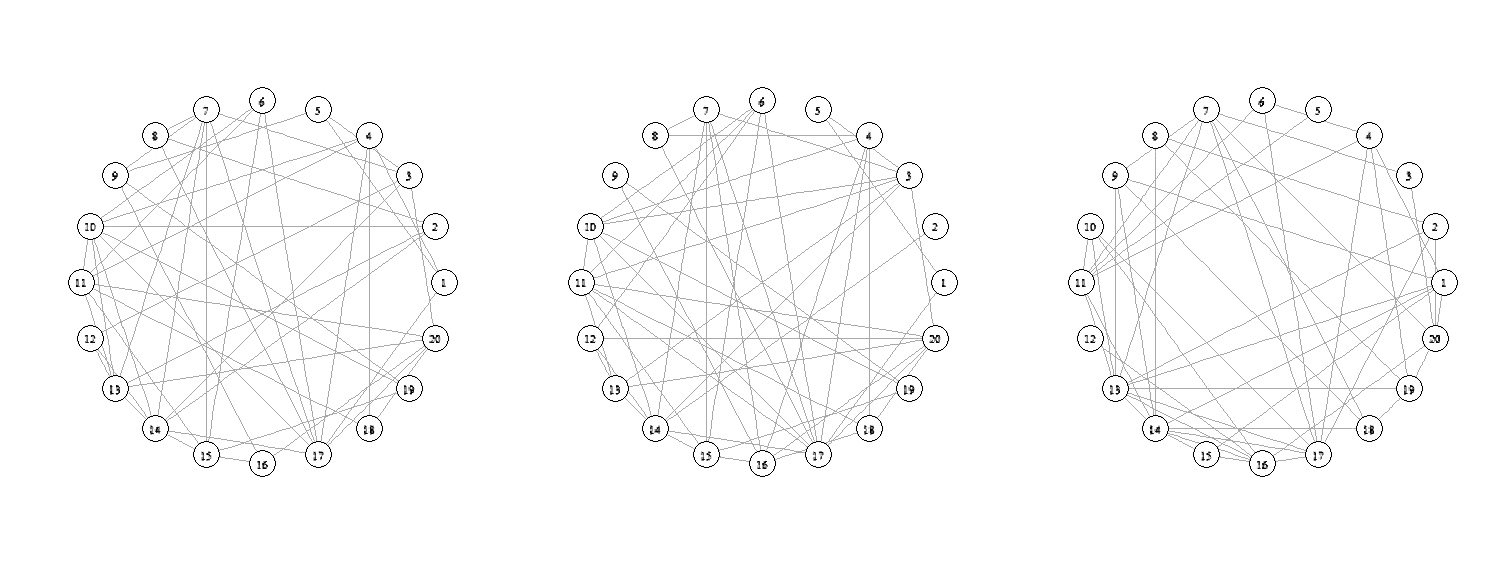
\includegraphics[width=1\linewidth]{ch-gc/figures/sim_10vs50}
		\caption[Random graphs with 20 nodes and 50 edges. Edges have been 
		swapped 10 and 50 times respectively.]{\textit{Left:} Base graph 
		$G(V,E)$ with $V=20$ nodes and $E=50$ edges.\textit{Middle:} Random 
		graph built from $G$ by randomly swapping 10 edges. \textit{Right:} 
		Random graph built from $G$ by randomly swapping 50 edges. 
		Distance: L2. Seed: 1000}
		\label{fig:gc:sim10vs50}
	\end{center}
\end{figure}

\subsubsection{Extensions}

Although the normalization methods proposed in Section~\ref{sec:gc:methods} 
have bounded the graph summarization values between 0 and 1, it does not 
necessitate that the values are uniformly distributed between 0 and 1. An 
alternative method of normalization leverages the XXXXXXXXXX to simulate a 
uniform distribution. A further extension would be to implement such a 
procedure, which is as follows:

\tablespacing
\begin{itemize}
	\item Simulate $n$ random graphs $G=(V,E)$. If implementing for the 
	simulation above, all simulated graphs would have $|V|=20, |E|=50$.
	\item Compute the difference between each pair of graph (or the base 
	graph???????)
	\item Find the $p$-value?????
\end{itemize}
\bodyspacing
